\renewcommand\evenpagerightmark{{\scshape\small Diagnostic}}
\chapter[Diagnostic and Methods]%
{DiagnosticMeasurement}
\label{diagnostic_chapt}

\section{Strioscopy}

\subsection{Opportunities}

What we would like to measure :

\begin{itemize}
\item velocity field
\item density field
\item turbulence field
\item mixture field
\item recirculation zone
\end{itemize}

What we are sure we can measure if the experiments works perfectly  :

\begin{itemize}
\item qualitative representation of the mixture
\item qualitative idea of the turbulence 
\item recirculation zone
\end{itemize}



\subsection{According to the user guide}

Possible to compute quantitatively the density, the temperature (assuming that we know the pressure), even some velocity values... It is very well described, the calculations are very long and not automatized in a script (feasibility?)

\section{Procedure}

\subsection{What is needed}

\begin{itemize}
\item The strioscopy
\item a dilution facility 
\item A thermocouple
\item A calibrated movable pedestal
\item A CCD camera (when the whole diagnostic is proven to work)
\item The preheater
\item An area of $4m * 2m$
\item Gaz supply (air?) at the right velocity
\item a table, a meter
\end{itemize}
\section{Dimensional analysis}
\subsection{The approach}
As far as it is possible, we want the adimensional numbers to remain the same: $\frac{d_{1}}{D}$,$\frac{d_{2}}{D}$,$Re_{1}$,$Re_{2}$,$S_{1}$,$S_{2}$,$J$ and $\frac{\rho_{1}}{\rho_{2}}$. We also want to use the same velocities as the ones in HPPOX. 

According to our hypothesis to consider the geometrical swirl number, we see that the use of the same ATR-30norm burner automatically gives that $\frac{d_{1}}{D}$,$\frac{d_{2}}{D}$,$S_{1}$ and $S_{2}$ remain the same. (Let us neglect in a first approach the fact that we will not use any combustion chamber in the strioscopy diagnostic, so that the diameter $D$ is not defined anymore). 

Hence, we have to choose our inlet gases in order to keep as constant as possible the quantities : $Re_{1}$,$Re_{2}$,$J$ and $\frac{\rho_{1}}{\rho_{2}}$. Unfortunately, other conditions make the conservation of these adimensional quantities all the more difficult :
\begin{itemize}
\item To increase the efficiency of the strioscopy, one needs a high density gradient, implying that we need   $\frac{\rho_{2}}{\rho_{1}}$ far from the unity. "far" still needing to be defined. By heating air at $100^\circ C$, Y. Joumani (ref) had a density ratio of 1.27, which apparently was not enough. Fortunately, since we want to approach $\frac{\rho_{1}}{\rho_{2}}$ from the experiment on Calhory, the value reaches $\frac{\rho_{O_{2}}}{\rho_{CH_{4}}}_{Freiberg}=3$ , which may be enough to have useful density gradients.
\item Dealing with the experiment, heating the gases or diluting them make the experiment more difficult to implement. Particularly, though it would be an efficient solution, using natural gas without combustion chamber nor furnace seems unsafe.
\end{itemize}

\subsection{The dimension calculation }
An Excel tool has been created to compare the HPPOX values and the strioscopy diagnostic. As a preliminary conclusion, the theoretical best option would be to use natural gas and air at ambient temperature. Since the unburnt natural gas may be forbidden, another option would be to use air/air and burn the inner air at $200 ^\circ C$ , the adimensional numbers would be quite accurate, except the inner Reynolds number$Re_{1}$. One can refer to the Excel sheet for more details. 

With Python, a parametric study may be conducted to explore all the possibilities and analyze if there is not a better option to match the adimensional numbers.

In order to mitigate the conclusion, since we do not expect, for now, a very accurate comparison, nor a very precise quantitative diagnostic, we may not need to respect these adimensional numbers with such an accuracy. 

\subsection{Operational concerns}

\begin{figure}[!h]
  \centering
\includegraphics[width=0.6\textwidth]{fig/Schema_strio.png}
  \caption{The strioscopy experiment}
 \label{schema_strio}
\end{figure}
\subsubsection{The diagnostic of strioscopy }

There many kinds of strioscopy, the global aim is to measure the difference of optical path between two coherent beams. A difference of optical path induce a difference of density according to Gladstone-Dale law : $n-1=\kappa  \rho$. 

The strioscopy available at CRCD is interferential strioscopy, whose principle is described here :
\begin{figure}[!h]
  \centering
\includegraphics[width=0.8\textwidth]{fig/Principe_Strio.PNG}
  \caption{The strioscopy diagnostic}
 \label{principe_strio}
\end{figure}
A mercury source light (S) polarized by a polarizer (P) is divided into two coherent beams with a 1st biprism (B1). If the optical path between the two beams are equal, the 2nd biprism (B2) will gather the two beams, so that the polarization plan will be the same as before. A second polarizer works as an analyzer (A) : it  has a polarization plan perpendicular to the 1st polariszer, so that if the beam is not modified, no beam will be transmitted through the analyzer.

In case of a difference of optical path in the volume we want to measure, the polarization plan of the beam leaving the second biprism (B2) will not be the same, and its projection on the perpendicular polarization plan of the analyzer (A) will not be equal to zero anymore.

A fringe set up can be obtained by translating the second biprism along x-axis : without any perturbation of the measurement volume, the difference of optical path is then going to depend on the coordinate of the beam, so that parallel interferential fringes will appear in the absence of  perturbation of the measurement volume. The fringe set-up is responsible for the observation on figure \ref{image_strio} : when there is no pertubation, the fringes are strictly parallel, we can here observe a boundary layer at the proximity of the solid body thanks to the disposal.

\begin{figure}[!h]
  \centering
\includegraphics[width=0.8\textwidth]{fig/Strioscopie.PNG}
  \caption{The strioscopy diagnostic}
 \label{image_strio}
\end{figure}


\subsubsection{Procedure}

\begin{enumerate}
\item On a table, install the strioscope device
\item install the spherical mirror 3 meters ahead the lens of the strioscope
\item To calibrate the device, you can : \begin{itemize}
\item control the translation of the optical device (particularly, two configurations can be reached (by moving the strioscope along the optical axe): flat-colour or with fringe, in the case of fringes, one can change the position of the fringes by moving the biprism laterally)
\item choose the angle of the biprism ($1^\circ$,$2^\circ $ or $3^\circ$)
\item control the movement of the refringent bi-prism
\item In order to make the focus : control the drum with 8 positions for lenses, and then adjust it manually with the secondary fine controlling button (at the end of that point, the focus is supposed to be done on the examined object)
\item Change the device on which the final image is reflected (it can be a dulled glass, or a photographic plate, or a camera fixed to a support, or a screen)
\end{itemize}
\item One can check the set up with a small flame from a lighter
\end{enumerate}
\subsubsection{To take into account}
\paragraph{Protect the flow from the wind} It is absolutely necessary not to be under the influence of the wind. The best option is to make it indoor.

\paragraph{Taking care with the outlet temperature} Y. Joumani had troubles with keeping the outlet temperature because of the cooling inside the pipe. We have to measure it at the outlet (with thermocouple, for every used mass flow!) but also to insulate the pipes, or preheat a lot the initial gaz.

\paragraph{To test if the burner is really axisymetrical} Turn the burner and compare the results

\subsubsection{To include in the planning}
\begin{itemize}
\item CCD camera
\item Preheater
\end{itemize}
\section{The sizing of the reheater for the strioscopy}

  This is a compromise between the need for the experiment and the difficulty to craft the facility. This is a problem of heat transfer : with a given mass flow $\dot{m}=20.5 kg/h$, we want to heat air from ambient temperature to $T_{outlet}=605^\circ C$ with a hoven of maximal temperature $T_{hoven}=850^\circ C$. A simple OD model gives the energy balance :
  
  $\dot{m} c_{p} (T_{outlet} -T_{inlet})=(T_{hoven}-T_{mixture}) h S_{wet}$
  
  We use the correlation heat transfer : 
  
  $h=0.023 Re^{4/5} Pr^{0.3}$,  we introduce the length :$x_{0}=\frac{c_{p} \dot{m}^{1/5}D^{4/5}}{\lambda Pr^{0.3} 0.023 (4/(\mu \pi)^{4/5}\pi}$ 
 
and we find with a 0D model the necessary length $L$ to reach the outlet temperature : $L=x_{0} \frac{T_{outlet} -T_{inlet}}{T_{hoven}-T_{mixture}}$ 

and with a 1D model : $L=-x_{0} ln(1-\frac{T_{outlet} -T_{inlet}}{T_{hoven}-T_{inlet}})$  

The figure \ref{heater_sizing} shows that the two models are quite close at 1st order, we have to choose a technical solution with a reliable velocity (less than 30). Margins has been taken in this scenario, knowing that the pipe will not be at the exact temperature of the hoven, and that we want to over heat the flow at the outlet to compensate the thermal loss to reach the burner.

\begin{figure}[!h]
  \centering
\includegraphics[width=0.9\textwidth]{fig/dimensionnement_rechauffeur.pdf}
  \caption{The heater sizing}
 \label{heater_sizing}
\end{figure}

Depending on what can be crafted, we may choose a 6meters long pipe of 20mm as internal diameter.

\section{Review of the use of Schlieren to study the jet}

The use of Schlieren as a diagnostic to study the jet. (\# ref Faivre and Thierry Poinsot) has used it to study the influence of the Swirl on the cone angle, describing the mixing. The major problem with Schlieren is the difficulty to interpret the signal. The intensity measures the quantity of density gradient the beam has crossed. It can be used to detect the edge of flows, as it is the case with cone angle with jet.
ref  Ben-Yeoshua used it also a lot, and considered that he was able to find the recirculation zone whis this diagnostic :



\begin{figure}[!h]
  \centering
\includegraphics[width=0.6\textwidth]{fig/CRZ_schlieren_these}
  \caption{CRZ captured by Schlieren}
 \label{Schlieren CRZ}
\end{figure}

\section{Acquisition of the flame}

The acquisition of the flame is the main experimental method to study the flame topology. Different optical diagnostics has been used. The visible signal of the flame has obviously been a first source of observation, but as it will be explained further, visible acquisition of the flame depends a lot on the parameter acquisition of the camera (time exposer, ISO sensibility, dynamic range of the sensor) and images are very difficult to study. Phenomena such as the formation of soot impedes from drawing conclusion on the flame topology with visible signal. The Hydroxide radical (OH), the Methylidyne radical (CH), and the Diatomic  carbon radical (C2) are intermediate species that can be encountered within the reaction front of hydrocarbon flames. The molar fraction of these three intermediate species depends on the nature of the input gas, and on the temperature reached in the front reaction. Guilberti \# ref gives more explanation in his work.

Among these intermediate species, some of theme are excited in a state noted *. Their spontaneous emission can be captured when they transit back to the ground state, and occurs at a specified wavelength. The principle of flame chemiluminescence is to capture their  emision by filtering the signal to the specific wavelength emission of the intermediate species to be observed. For $OH^*$ and $CH^*$ excited species, the peaks of spontaneous emission are respectively $309nm$ and $431nm$ at certain conditions of temperature. Narrow-bandpass filters are placed between the flame and the camera. Though $OH^*$ emits much more than $CH^*$, the optical devices decreases a lot the UV-signal so that their emissions is of the same order.(\# guilberti). To capture $OH^*$ emission, the camera needs to capture the UV light, and all the optical devices has to be transparant with UV. This is the reason why $OH^*$ diagnostic has not been conducted with the endoscope.

The filtering of the signal recquires an intensified camera for $OH^*$ detection, and a high sensibility camera for the $CH^*$ signal. Here are the equipment used :

\begin{itemize}
\item ANikon D600 (http://www.sensorgen.info/NikonD600.html)
\item A Pi-Max 5 camera (\#ref)
\item Endoscope
\end{itemize}
 




\section{Comparison between OH*, CH* and visible light}
\subsubsection{The difficulty of using the visible signal}
Though the optical diagnostics have been studied to compare the signal at different wavelengths in the internship, I reckon that a detailed study would be needed to study in depth the signal provided with  $OH^*$, $CH^*$ and visible signal. In the context of the internship, different diagnostics has been used for practical reasons, considering that the $OH^*$ signal captured by the intensified light would always be the best option. As it has been said, the intensified camera could not be used with an endoscope, so that flame longer than $120 mm$ could not be wholly captured. This is the major reason why $CH^*$ and visible signal has been used, the second being the fact that the intensified camera has been available for a certain lapse of time.

The bottom line of the internship is to study the flame at an infinite-rate chemistry, thus considering the flame only as a stoichiometric line. In this ideal scenario, the excited species, whose life time is short, are mainly situated in the flame front (they are produced at the stoichiometry, and their lifetime tends to be zero as the flame is considered as infinite-rate chemistry). Hence, $CH^*$ and $OH^*$ signals corresponds much more to what the front flame than the visible signal. Indeed, depending on many criteria, the flame can produce more or less soot : diluting the natural gas with nitrogen tends to reduce the soot production; similarly, a flame with a very high momentum flow ratio tends to produce less soot. In order to show to what extent the signal can differ, the figure \ref{fig_comparison_soot} compares the instantaneous signal of rich soot flame (left), a nitrogen diluted flame (middle) and a high momentum flame (right), all recorded with the prototype burner in the visible light.

Eventually, the visible signal depends on the parameter acquisition of the camera, and also on the soot formation, my conclusion is that the visible light cannot be used to calculate flame length. However, it seems that the industrial flame lengths are often sized with visible light (Optysos). 

\begin{figure}[!h]
  \centering
\includegraphics[width=0.3\textwidth]
{fig/soot/soot_rich.jpg}
 \includegraphics[width=0.3\textwidth]
 {fig/soot/high_N2.jpg}
  \includegraphics[width=0.3\textwidth]
 {fig/soot/high_M.jpg}
  \caption{Here are three flames from the prototype burner, showing the difference of signal due to the soot radiation : left :  rich soot flame with medium flow momentum ratio, middle : nitrogen dilluted flame, righ : pure natural gas flame with high flow momentum ratio }
 \label{fig_comparison_soot}
\end{figure}
\subsection{Comparison between CH* and OH* signal}

\section{Post-processing of the flame}

The purpose of this section is not only to show that a lot of endeavors have been accomplished to post-treat the data, but also to prove the 
reliability of the results to be given in the next chapter  \# ref chapter!!!!. 
\subsection{The diagnostic and their flame length}

Though measuring the distance seems trivial, it is becomes very complicated in a $500^\circ C$  furnace, where the desired accuracy is a few millimeters, in a 6 meters long furnace. The main difficulty has always been the lack of optical access of the furnace, as it can be seen in picture \ref{fig_calhory_furnace}. The furnace has not been designed so as to study the flame shape nor length, it has been an everyday challenge to picture all the signals with the different acquisition parameters.

 \begin{figure}[!h]
  \centering
\includegraphics[width=0.45\textwidth]{fig/com/four.JPG}
  \caption{The Calhory furnace}
 \label{fig_calhory_furnace}
\end{figure}

The flame from Optysos report were less than $150 mm$. So 150 mm capture in the furnace could be enough. Unfortunately, one must consider that :
\begin{itemize}
\item the post-processing uses Otsu tresholding, so that the full flame needs to be taken (and not only the edge of the flame), since the peak of intensity of the flames needs to be captured so that the threshold is efficient (this can be seen further in figure \ref{fig_Iso_sensitivity_1D}
\item The flame must not reach the edge of the volume area, since the threshold has ta take into account the full decrease of intensity from its peak to its end
\end{itemize}
The $OH^*$ diagnostic with the intensified camera only took a $120mm$ long signal, which was only significant from flame measuring less than $120mm$. The intensified camera has not been used with the endoscope since the endoscope does not transmit the UV signal. But the endoscope has been used for the $CH^*$ signal and the visible, and flames of length as far as $240 mm$ have been reached.
\subsection{The geometrical transformations with the use of a calibration rod}


 \begin{figure}[!h]
  \centering
\includegraphics[width=0.45\textwidth]{fig/com/rod_entering.JPG}
  \caption{The calibration rod}
 \label{fig_rod_entering}
\end{figure}

When using an endoscope, the accumulation of optical devices and the law of perspective morphs the image, so that the output image has to be sized, scaled, and shaped. To that purpose, a calibration rod has been used : a graduated rod has been made, with plumb lines every 10 millimeters. The rod could enter in the burner tub when the furnace is cold enough, as it is show in figure \ref{fig_rod_entering}. The plumb lines falling with gravity, we can take an image of our well known calibration road, where the vertical and horizontal lines are graduated to create a $2D$-mesh grid in the vertical plan of the burner, where the flame is to be studied. 

Hence, from that acquisition of the 2D-grid, a Matlab geometrical script has been created, in order to transform the 2D grid from the endoscope into a real 2D grid, where the parallelism and the angles are respected. As it has commonly used in this field (\# ref thib guilberti), the Matlab function \textit{imtransform} is used, with projective transformations for the parallism, and piecewise for the graduation. The output of the whole procedure is a list of nine geometrical transformations that transform a distorted image into a fine shaped and sized image. If the nine geometrical transformations works on the calibration rod, they work specifically to the flame acquisition if the camera has not moved at all. 


The figure shows the main steps to transform an perspective image into a well defined grid. To the purpose of the exercise, an over distorted image of the calibration rod has been taken, to show the efficiency of the calibration code. It can be observed at the last picture that the graduation are regularly spaced out, and correspond to the good indication in millimeters (one graduation on the physical calibration road is 25 mm, it can be checked that this is correct on the final picture).

Even with a lot of distortion, as it is the case with the previous picture which makes a high angle with the calibration road, the transformations gives a fine sized shaped picture. The accuracy of the process is very good, pointing the graduation of the rod on the final plot gives a deviation of less than 1\% between the indicated distance and the real distance on the rod.
\begin{figure}[!h]
  \centering
\includegraphics[width=0.6\textwidth]{fig/Matlab_calibration.pdf}
  \caption{From up to down, left to right : Step 0, raw image from endoscope; step 1, lines of perspective supposed to be paralleled; step2, correspondency to re-establish paralellism; step 3 : results of the transformation, step 4 : cropping; step 5; the horizontal graduation are used to make the horizontal scaling, using a piecewise transformation;step 6 the vertical gradution of the plumb line are used to scale the vertical direction }
 \label{fig_timetable}
\end{figure}

\subsection{Timetable of a typical day}

As it has been said, it was an absolute necessity that the camera did not move an inch to apply the geometrical transformations to the flame acquisitions. Hence, acquisitions of the calibration rod were takin in the morning and in the evening. The criteria to testify the results of the acquisitions of the day was that the calibration rod where exactly at the same position in the morning picture and in the evening picture. Fortunately, this has been verified every day (meaning that no data were lost because of a fortuitous move of the camera or the endoscope).
\begin{figure}[!h]
  \centering
\includegraphics[width=0.6\textwidth]{fig/com/timetable.png}
  \caption{Typical day}
 \label{fig_timetable}
\end{figure}

\subsection{Validation of the post-processing}
In this section, the problem of the acquisition parameters is addressed. To what extent the flame length result depends on the acquisition parameters of the Camera? A few days have been spent to validate the acquisition treatment and the post processing. Comparing to Air Liquide practices, the flame length results presented here are way more reliable.  
\subsubsection{ISO sensitivity}
In this section, it is shown that with CH* and OH* detection, very good results have been obtained in terms of reliability, as it is not the case with the visible light.
\subsubsection{With CH*}
 
 With CH* filter, the two flames $ISO_{A} $ and $ISO_{B}$ are studied, here are the averaged intensity of OH*, uniformed from 0 to 1.  The purpose here is not to compare the flame but to study the influence of the acquisition parameters on the flame length.
 
 \begin{figure}[!h]
  \centering
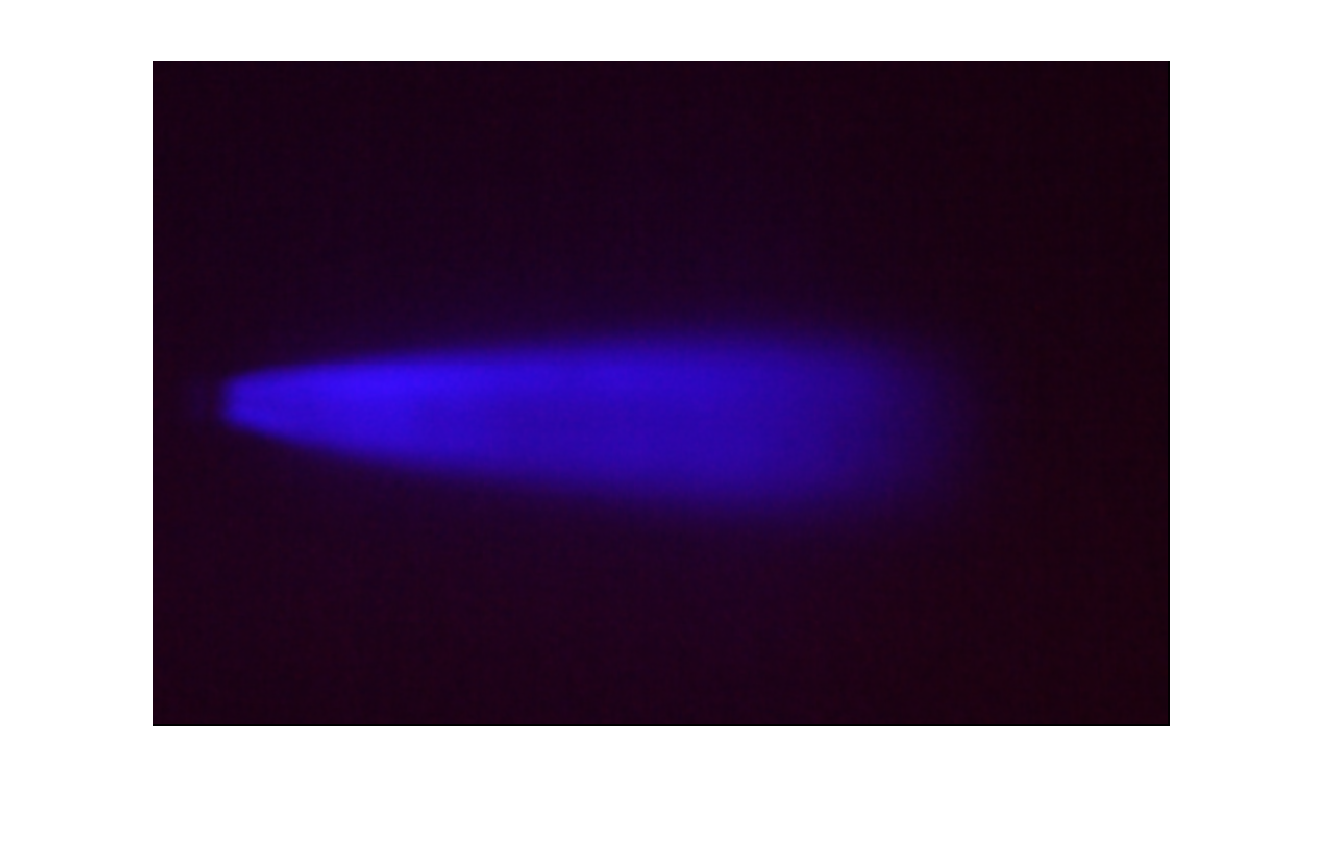
\includegraphics[width=0.45\textwidth]{fig/sensitivity/brute_4069.eps}
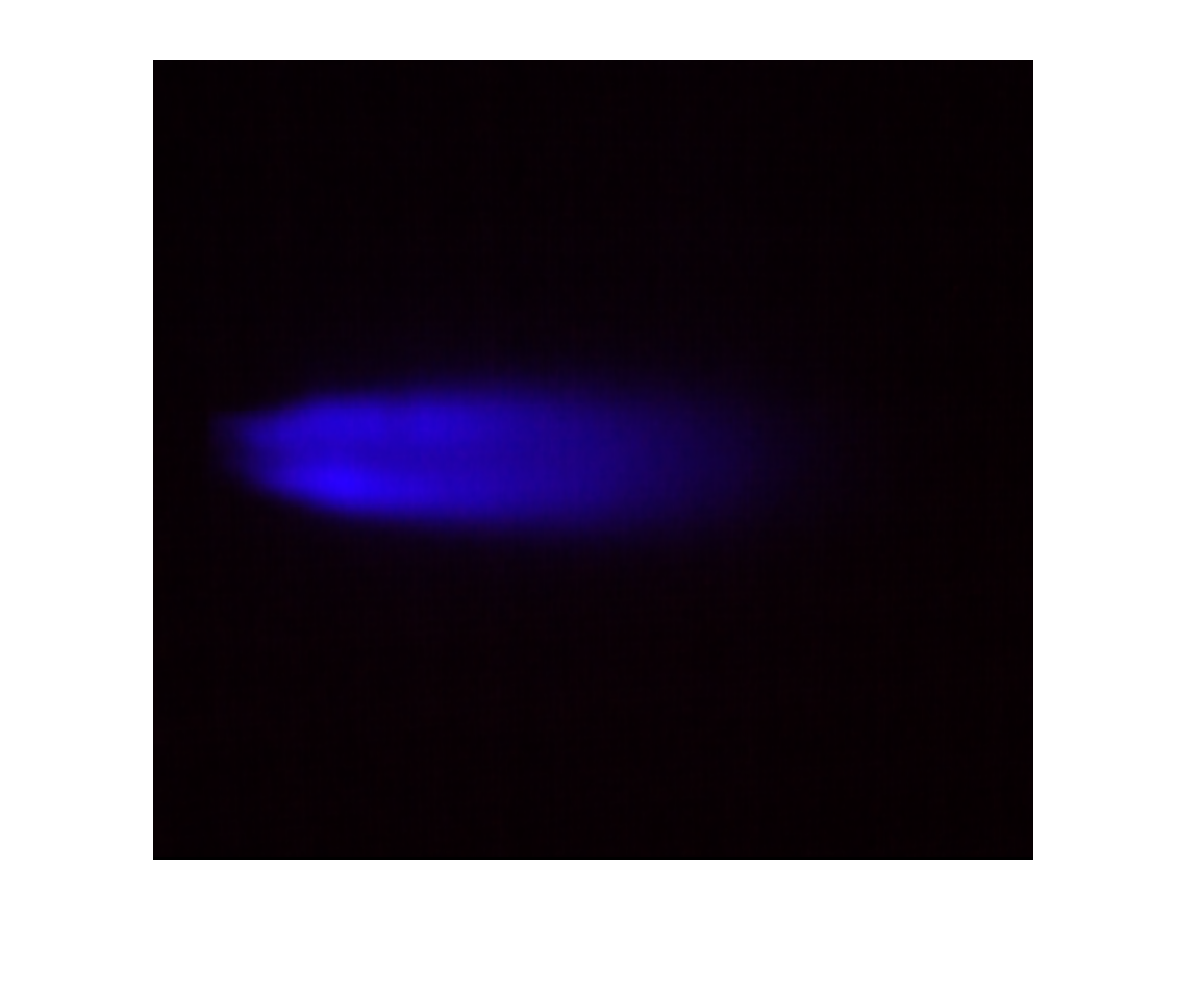
\includegraphics[width=0.35\textwidth]{fig/sensitivity/brute_4476.eps}
  \caption{Averaged $CH^*$ signal of two flames. On the left : $ISO_{A}$, Prototype burner, $X_{1,CH_{4}}=0.75$, $M =0.731$,$S=0$. On the right : $ISO_{B}$, ATR burner, $X_{1,CH_{4}}=0.5$, $M = 1.438$}
 \label{fig_ISO_brute}
\end{figure}
 
The objective of the post-processing is to test for each measurement, that the acquisition is in the area where the flame length does not depend on the ISO sensitivity of the camera. There are two requirements to achieve so :
\begin{itemize}
\item The signal must not be saturated at all (i.e. the maximum capture by the image must be less than 255 in RGB format)
\item The signal must not be too low, otherwise only the peak of signal can be detected, and not the rest of the picture.
\end{itemize}
Dealing with the saturation, the post-processing treatment always calculated the maximum of intensity in the image to be sure that it was not saturated. From now on, all the images shown are not saturated (the color have been re-scaled, so that the maximum displays 1, but the acquisition images has been checked for all the images).
\begin{figure}[!h]
  \centering
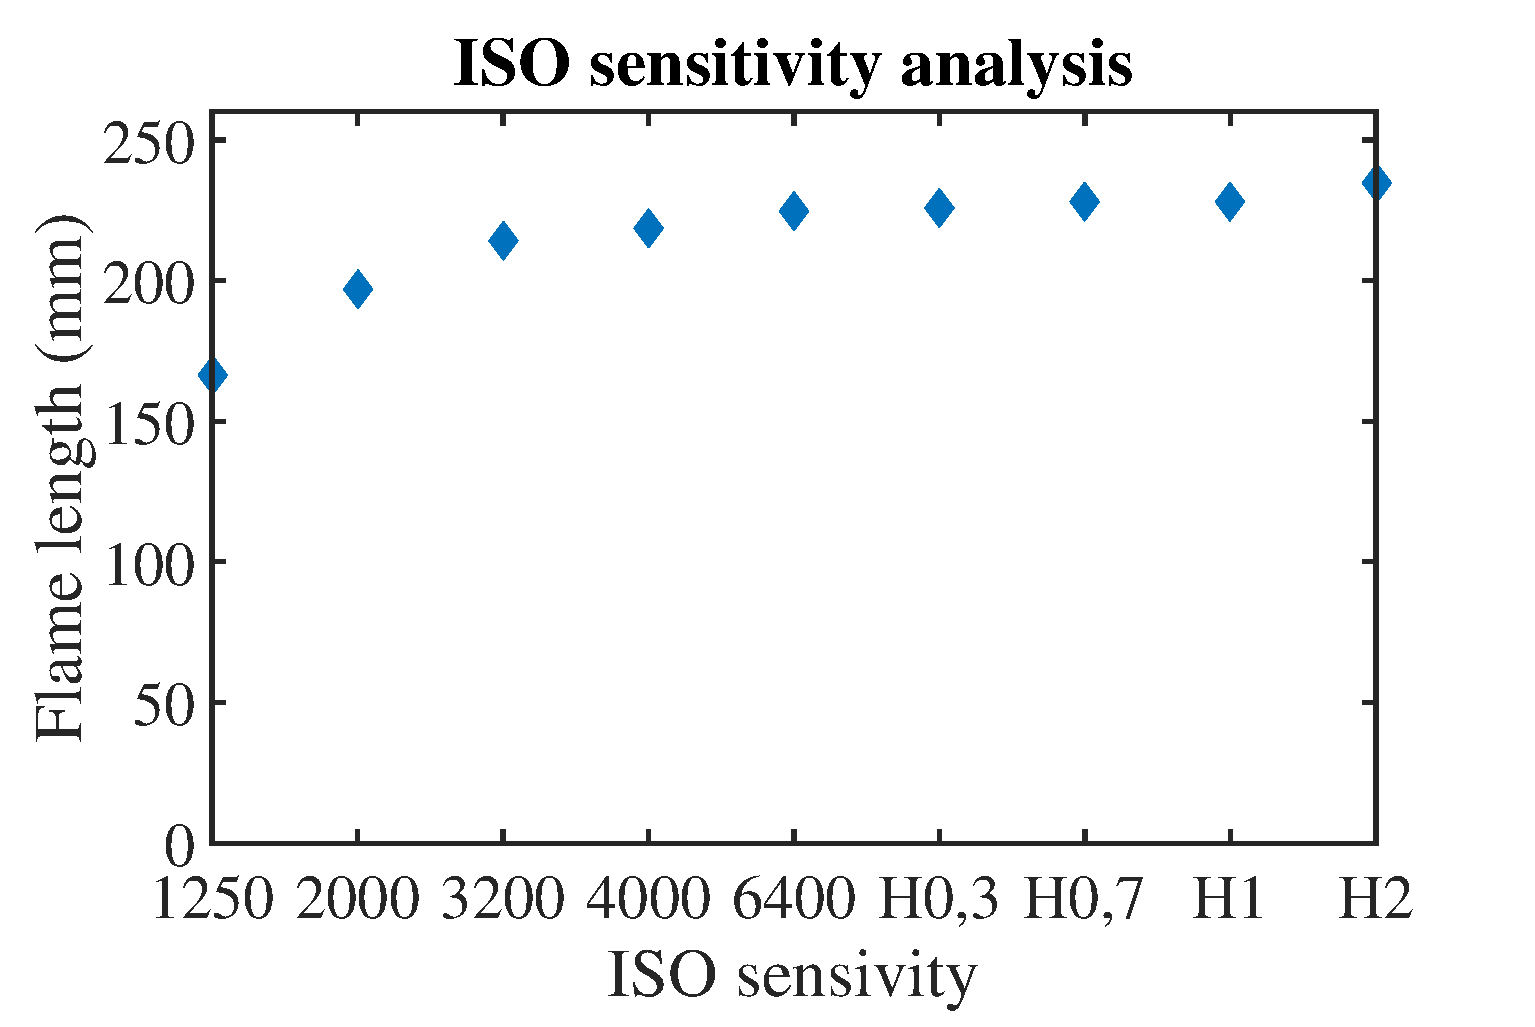
\includegraphics[width=0.4\textwidth]{fig/sensitivity/ISO_sensivity_analysis_4069.eps}
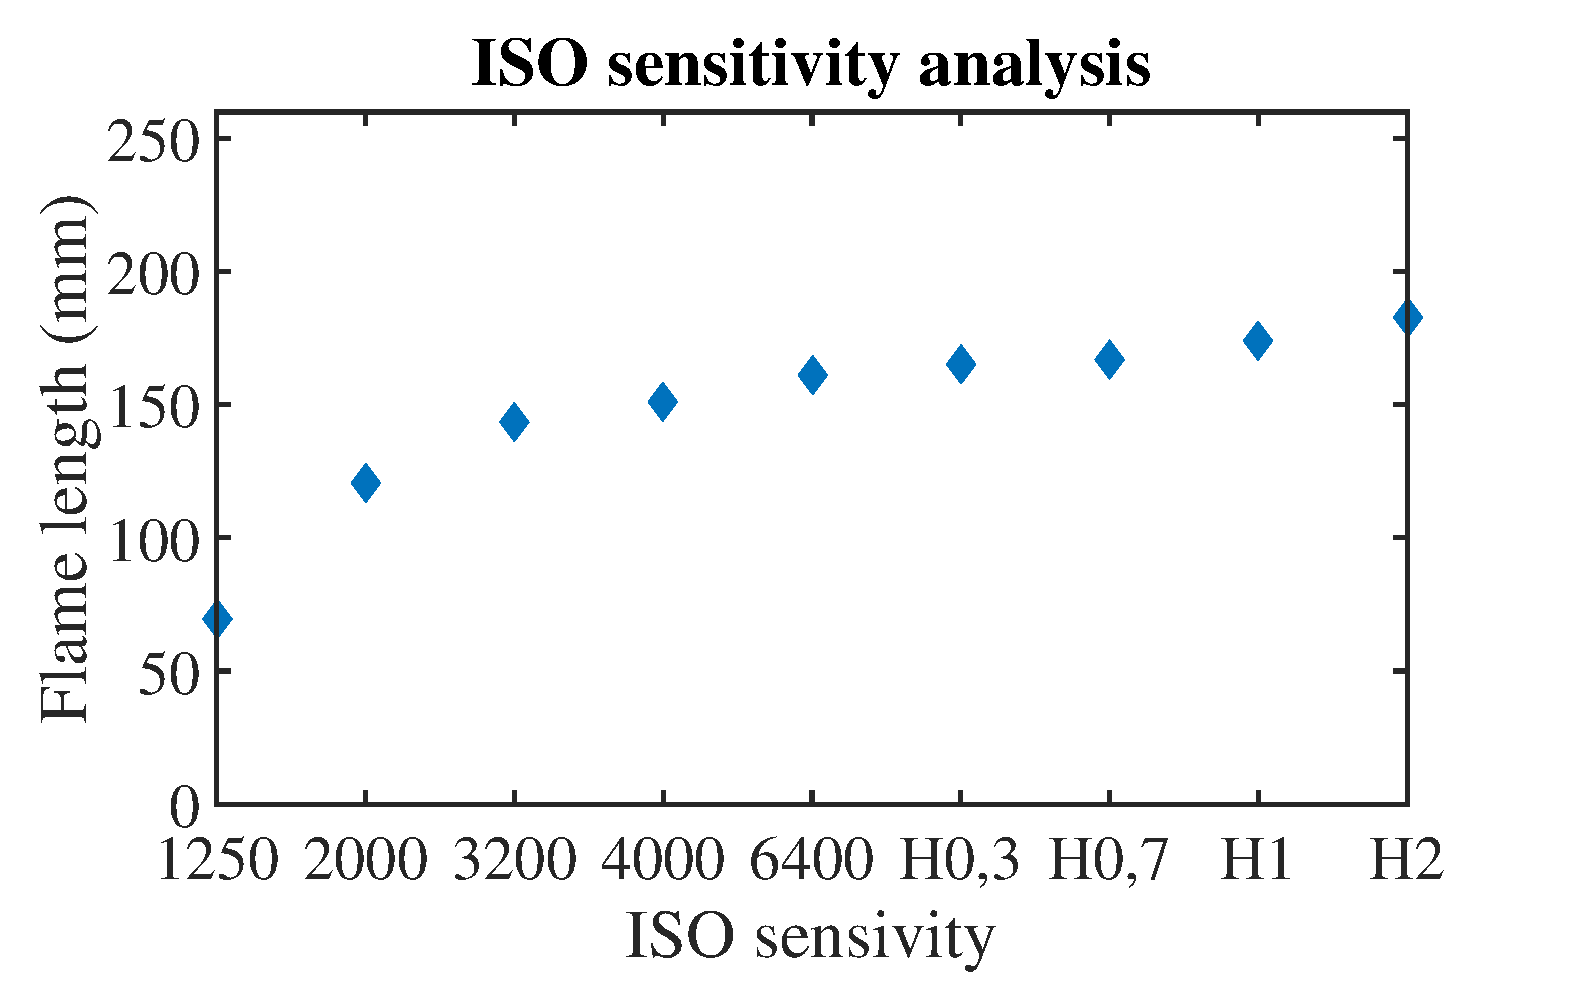
\includegraphics[width=0.4\textwidth]{fig/sensitivity/ISO_sensivity_analysis_4476.eps}
  \caption{Typical ISO sensitivity}
 \label{fig_Iso_sensitivity}
\end{figure}
Unfortunately, the signal being the luminosity through the CH* filter, the intensity of the signal depends a lot on the flame (CH* production, dilution effect...). It has been observed that, when the $CH_{4}$ is diluted with $N_{2}$, the intensity signal is lower.
Consequently, the post processing is less efficient when the ISO sensitivity decreases (as it is show in figure \ref{fig_Iso_sensitivity}). It can be seen that the curve is less flat, so that the accuracy of the post processing giving the flame length decreases when N2 dilution occurs. However, all the efforts have been made in order to check that the acquisition points have been taken at an ISO sensitivity high enough to been in the "flat area" of the sensitivity. Furthermore, although the figure \ref{fig_Iso_sensitivity} tackles the accuracy of the given flame length, one must consider that a flame acquisition with a CH* filter and less than 3200 ISO gives a black screen that would never have been shot if the ISO sensitivity anlysis would not have been done. Being said differently, capturing a visible signal on the Camera (that is not saturated) with a CH* filter still gives pretty good results, and prevents from being in the area where the flame length depends too much on the ISO sensitivity.

\subsubsection{An explication with 1D plot}
Even if the intensity of the acquisition signal can change, the post-processing (and the Odsu threshold) would be supposed not to deal with strict values, but with the shape of the signal after its standardization. So it must be explained why the flame length slightly changes when varying the ISO sensitivity. The figure \ref{fig_Iso_sensitivity_1D} gives the answer, here are plotted the signal intensity of the post-treated flame along the axis of symmetry. The flame is always extracted from more than 100 pictures, then averaged, then uniformed so that that the signal goes from 0 to 1. The different curves correspond to different parameters of acquisition of ISO sensitivity.

From a certain value of ISO, the shape is very comparable, whereas it differs when the ISO decreases under 3200. Besides on can observe that :
\begin{itemize}
\item The maximum of intensity is always at the same position no matter the ISO sensitivity. So that the maximum of intensity completely defines a performance of the flame, and does not depend at all on the parameters acquisition
\item Even with the standardization, the 1250 ISO signal is almost a black picture, so that it is clearly shown that the post-treatment is not to be blamed for  the inaccuracy of the flame length at low ISO , but a drastic lack of signal
\end{itemize}




\begin{figure}[!h]
  \centering
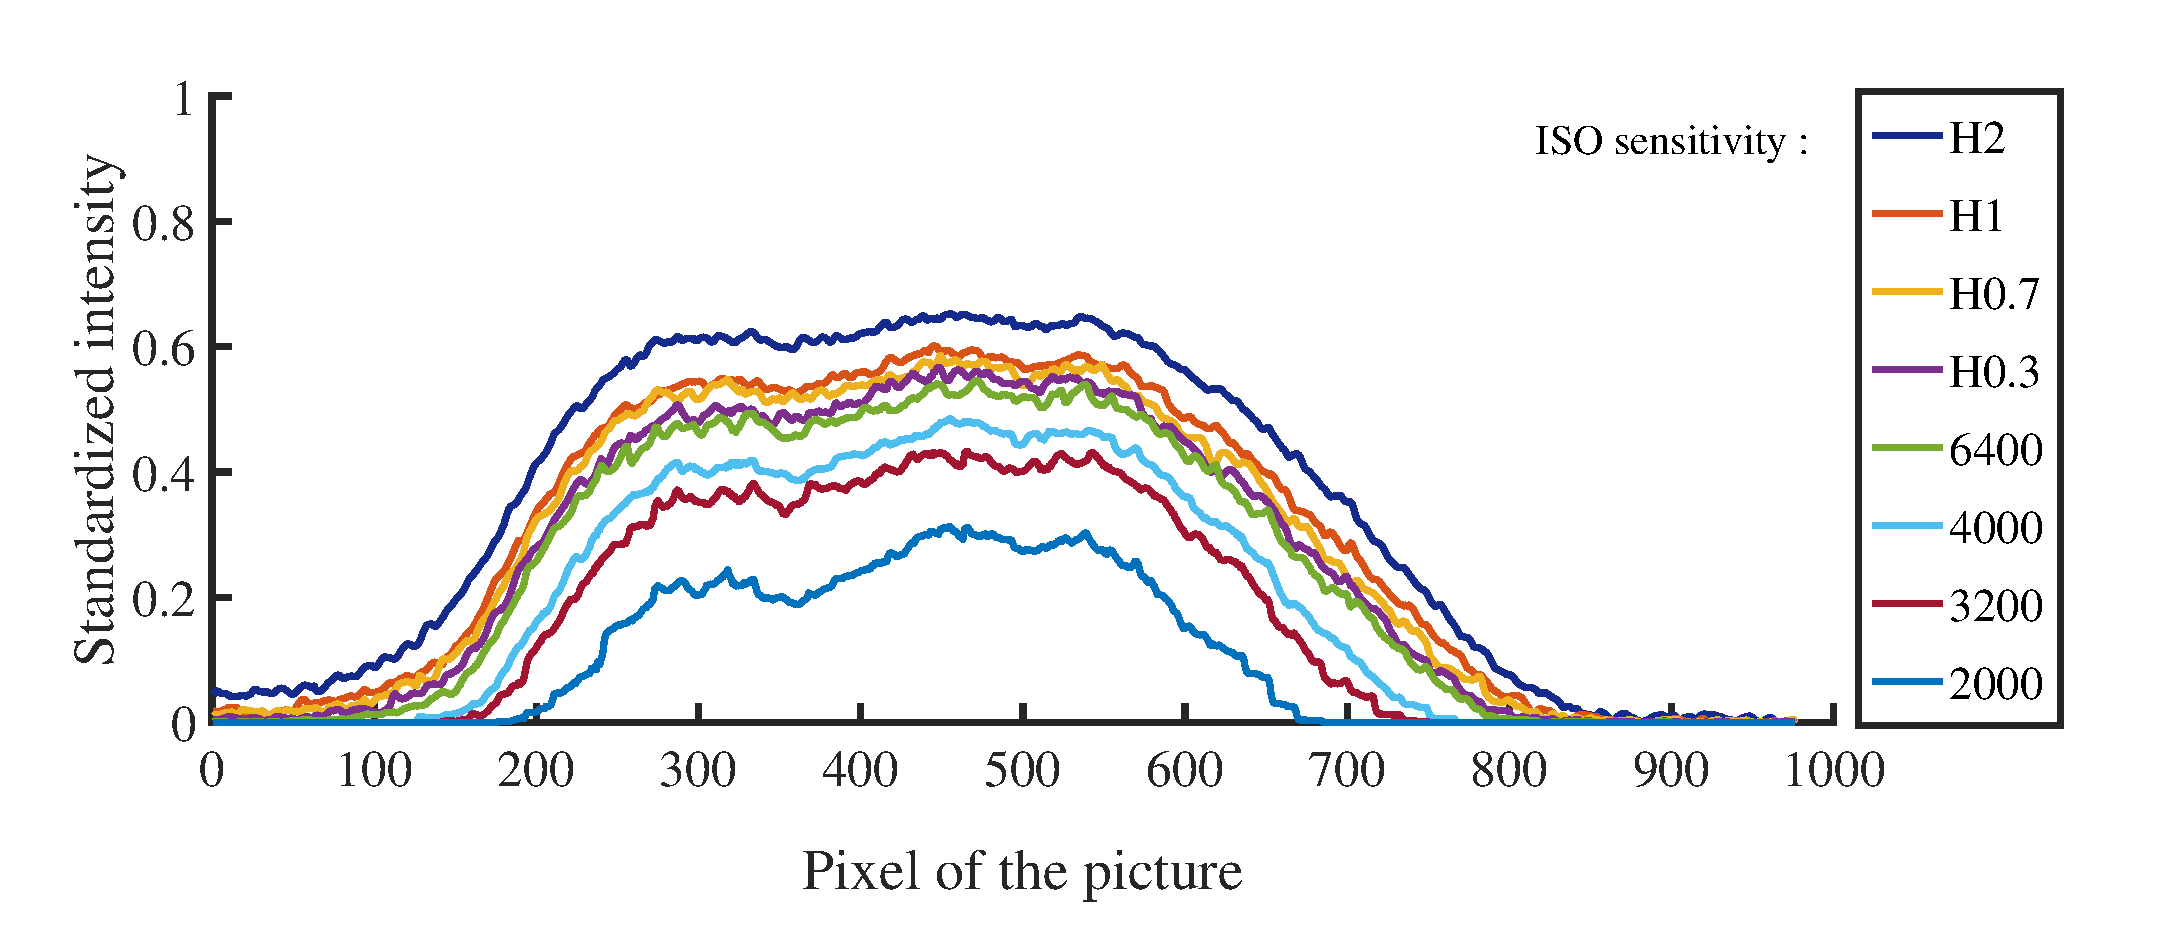
\includegraphics[width=0.40\textwidth]
{fig/sensitivity/1D_axy_4069.eps}
 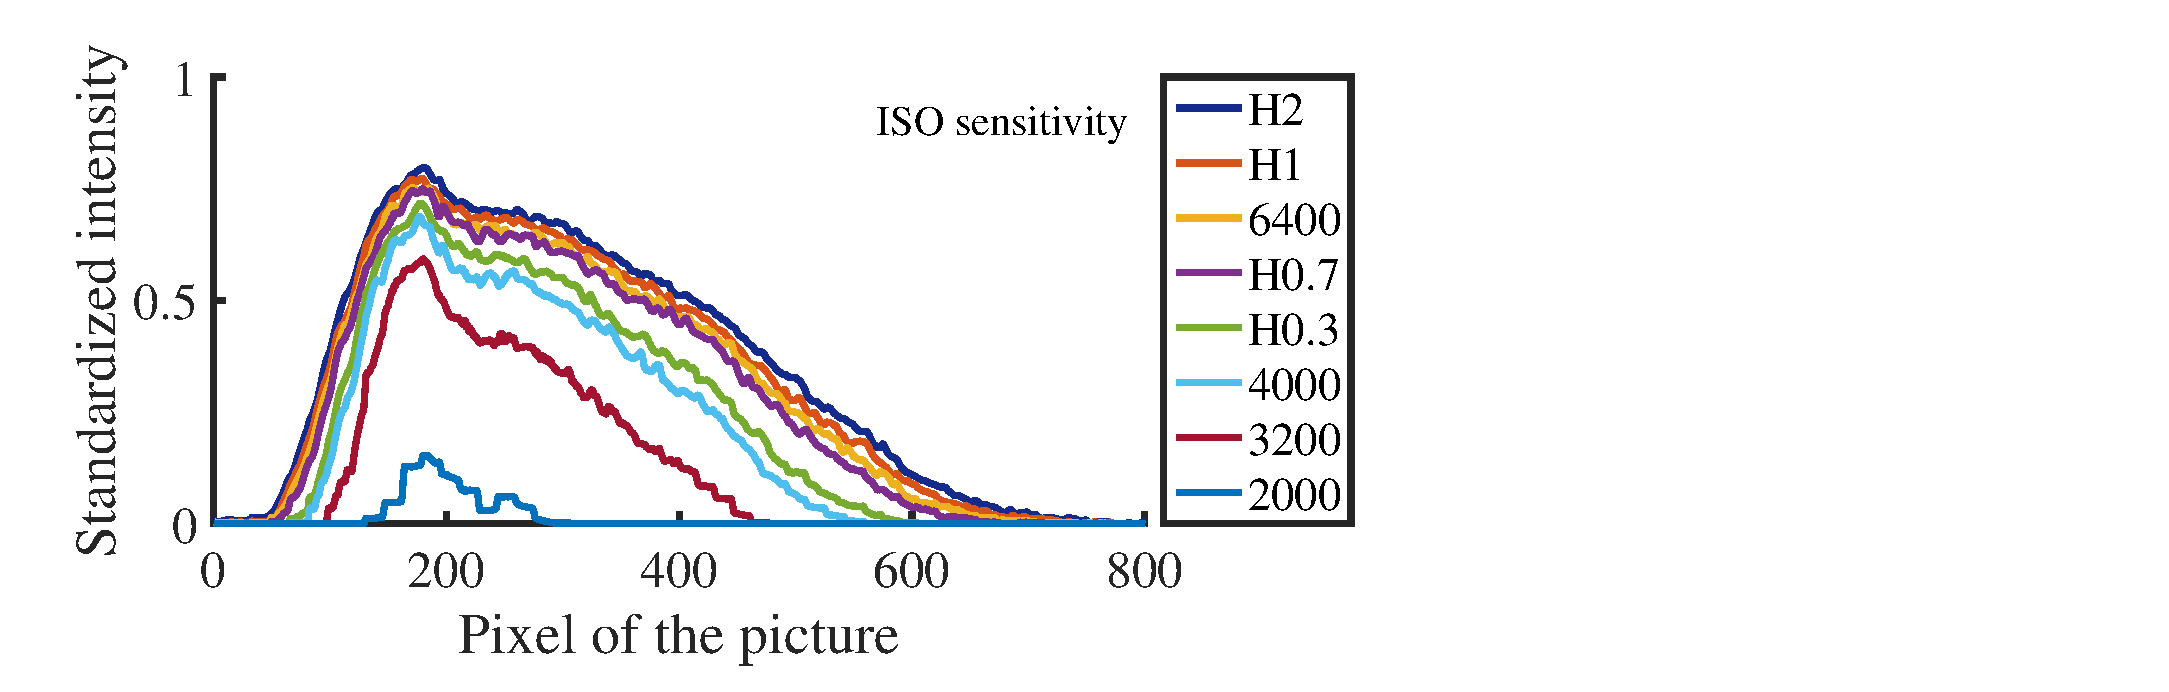
\includegraphics[width=0.55\textwidth]
 {fig/sensitivity/1D_axy_4476.eps}
  \caption{Typical ISO sensitivity}
 \label{fig_Iso_sensitivity_1D}
\end{figure}

\subsubsection{Digression on the functioning of a digital camera}
Furthermore, the impossibility to capture the right signal at low ISO is due to the encoding of a JPG picture. Indeed, the dynamic range of a JPG picture is very poor. A JPG picture being encoded in 8 bit, the signal goes from 0 to 255, and the signal between 0 and 1 is completely lost, as it is the case in figure \ref{fig_Iso_sensitivity_1D}. Unfortunately, there are two reasons why JPG format has been used :
\begin{itemize}
\item videos have been taken to average. It has been chosen to take a lot of flame acquisition, so the movie permits to have a quick acquisition, opposite to the burst mode, where the its takes more time to write in RAW format.
\item At the time, I did not find a proper way to work with NEF file in Matlab
\end{itemize}

After the acquisitions, I first regret having chosen JPG format. However, at the end, it may would not have changed to use NEF file instead of JPG file. Indeed, when converting the electron signal to a numeric signal, the error does not depend on the ISO sensibility. The website (\# REEF http://www.sensorgen.info/NikonD600.html ) gives data for the digital camera. The error of or writing in electron is approximately constantly 3 electrons for a saturation that depends on the ISO, giving a Digital Range of 256 when ISO is 6400. Hence, no matter the format used (RAW or JPG), the Dynamic range at high ISO almost impedes from working with high definition color file.

One of the way to prevent from this problem is to use an intensified camera, who multiplies the flow of electron (the analogical signal). Hence, the numeric error remains low compared to the intensified signal. For the Pi-Max 5, we can read \# ref PIMAX5 that the error is 8 electrons rms for 500 000 electrons, that gives a dynamic range of $DR=500k/8 = 62 500\sim 16 bit$. This is the reason why the problem of gain sensibility does not occur with an intensified camera.

sensor of the camera is still the same. So increasing the ISO sensibility decreases a lot the digital dynamic range. To a certain ISO, working with a 3200 ISO gives a signal over noise ratio so poor than it can be enough to work with 8 bit. 
